\section{拟映射墙交叉 (Yang Zhou)}%
\label{sec:Quasimap wall-crossing (Yang Zhou)}

本讲的主要墙交叉定理与主空间构造来自~\cite{Zhou2022}。 earlier 属零与高属结果见~\cite{CFK2014,CFK2020}，稳定拟映射的基础见~\cite{CFKM2014}。

设 \(X\) 为五次三维流形。我们的目标是计数 \(X\) 上的属零曲线，这个问题已由 Givental 与 Lian-Liu-Yau 解决。经由闭浸入 \(X \subset \P^4\)，可写出
\[ \bar{M}_0(X, d) \subset \bar{M}_0(\P^4, d), \]
它是光滑的并带有 \((\C^{\times})^5\) 的环面作用。若一映射被此作用固定，则定义域必有一些分支映到不动点，另一些分支构成一维轨道的 \(n:1\) 覆盖。特别地，不动轨迹由一组图来标号。

在此情形下，有量子 Lefschetz 原理，即
\[ [\bar{M}_0(X, d)]^{\on{vir}} = e(E) \cap [\bar{M}_0(\P^4, d)]. \]
此处向量丛 \(E\) 定义为
\[ E = \pi_* f^* \mc{O}(5), \]
其中 \(\pi\) 为万有曲线，\(f\) 为万有稳定映射。若
\begin{align*}
    I(q, z) &= 1 + \sum_{d > 0} \frac{\prod_{k=1}^{5d} (5H+kz)}{\prod_{k=1}^d (H+kz)^5} q^d \in H^*(X)[z^{-1}] \ps{q} \\
    &= I_0(q) \cdot 1 + I_1(q) \frac{H}{z} + I_2(q) \frac{H^2}{z^2} + I_3(q) \frac{H^3}{z^3},
\end{align*}
则
\[ J (Q, z) = 1+ \sum_{d>0} \phi^{\alpha} \ab<\frac{\phi_{\alpha}}{z(z-\psi)}>_{0,1}^X Q^d = \frac{I}{I_0} \]
在镜像映射 \(Q = q \exp\ab(\frac{I_1}{I_0})\) 之下成立，对此结果我们将给出不同视角。

\subsection{朴素计数}%
\label{sub:Naive counting}

我们考虑从固定的 \(\P^1\) 出发的“映射” \(\P^1 \to X \subset \P^4\)。为简单起见，设 \(X = \ab(\sum x_i^5 = 0)\) 为 Fermat 五次型。它由一组 \([f_0, \ldots, f_4]\) 给出，其中 \(f_i \in \C[u,v]\)，满足 \(\deg f_i = d\) 且 \(\sum f_i^5 = 0\)。要成为真正的态射，需要 \(f_i\) 无公共零点，但此模空间不正规，故放宽该条件。于是考虑模空间
\[ QG(X, d) =  \ab\{ [f_0, \ldots, f_4] \middle\vert \Vectorstack{{ f_i \in \C[u,v] } { \deg f_i = d }}, \sum f_i^5 = 0, (f_0, \ldots, f_4) \neq (0,\ldots, 0) \} \bigg/ \C^{\times}. \]
它位于到射影空间的有理映射的相应模空间
\begin{align*}
    QG(\P^4, d) &\coloneqq  \ab\{ [f_0, \ldots, f_4] \mid f_i \in \C[u,v], \deg f_i = d, (f_0, \ldots, f_4) \neq (0, \ldots, 0) \} \\
    &\cong \P^{5d+5-1} 
\end{align*}
之中。存在两个问题。第一，定义域是参数化的，故须计入 \(\P^1\) 的自同构。第二，为得到稳定映射，需将定义域爆破。

首先，令 \(\C^{\times}\) 通过伸缩 \(u\) 作用于 \(\P^1\)。考虑特殊不动轨迹 \(F_{\star} \subset QG(X, d)\)，定义为
\[ F_{\star,d} = \ab\{ [f_0, \ldots, f_4] \text{ fixed and } (v=0) \text{ is not a common zero} \}. \]
因此 \(F_{\star,d} = \ab\{ [a_0 u^d, \ldots, a_4 u^d] \mid [a_0, \ldots, a_4] \in X \} \cong X\)。从此角度出发，可用形变理论中的标准论证将 I-函数改写为
\begin{align*}
    I(q,z) &= \sum_{d > 0} \ab(\frac{[F_{\star, d}]^{\vir}}{e_{\C^{\times}}(N^{\vir})})^{\mr{PD}} q^d \\
    &= 1 + \sum_{d > 0} \ab( \frac{[X]}{e_{\C^{\times}}(N^{\vir})})^{\mr{PD}} q^d
\end{align*}
它位于 \(H^*_{\C^{\times}}(X) \ps{q}[z^{-1}]\) 中。

\subsection{非严格的墙交叉}%
\label{sub:Wall-crossing without rigor}


其次，考虑带有一个标记点加一条尾部并带有 \(\C^{\times}\) 作用的节点曲线 \(C\)，设有一映射 \(f \colon C \to X\)。若取极限
\[ \lim_{t \to 0} [f_0(t^{-1}u, v), \ldots, f_4(t^{-1}u, v)] = [a_0 u^{d_0}, \ldots, a_4 u^{d_0}], \]
则可见气泡的极限落入 \(F_{\star, d_0}\)，其中公共零点远离节点。于是可将此尾部替换为携带 I-函数某些项的新标记点。对五次型而言，这无非是 \(I_1 H - I_0 \psi = [zI-z]_{+, z = -\psi}\)。在此过程结束时，剩下 \(C = \P^1\) 带有 I-函数的各种贡献。

注意，若考虑 \(\C^{\times}\) 作用于 \(\P^4\)，则 \(f \colon C \to \P^4\) 被固定是指对一切 \(t \in \C^{\times}\)，存在 \(\varphi_t\) 使下图
\begin{equation*}
\begin{tikzcd}
    C \ar{r}{f} \ar{d}[swap]{\varphi_t} & \P^4 \\
    C \ar{ur}[swap]{t \cdot f}
\end{tikzcd}
\end{equation*}
交换。因此，我们在定义域上得到 \(\C^{\times}\) 作用。

我们将定义到 \(X\) 的 \(\ep\)-稳定拟映射模空间 \(Q_{g,n}^{\ep}(X, d)\)，它类似于稳定映射的模空间。我们希望把这些模空间看作彼此虚拟双有理，每个都是带完美阻碍理论的正常 DM 栈，从而可定义拟映射不变量
\[ \ab< \gamma_1 \psi_1^{a_1} \cdots \gamma_n \psi_n^{a_n}>_{g,n}^{\ep} \coloneqq \int_{[Q_{g,n}^{\ep}(X,d)]^{\vir}} \prod_{i=1}^n \ev_i^*(\gamma_i) \psi_i^{a_i}. \]
此处 \(\ep \in \Q_{>0}\) 为正有理数。可能的 \(\ep\) 空间具有墙-腔结构，墙出现在正整数 \(n\) 的 \(\frac{1}{n}\) 处。当 \(\ep > 1\) 时得到 Gromov-Witten 理论（即稳定映射），向左移动时，允许的有理尾部减少而基点增多。最终在 \(\ep \to 0^+\) 极限中，不允许任何有理尾部。最后，在 \(\frac{1}{d_0}\) 处的墙附近得到如下墙交叉公式：
\[ \ab<->_{g,n,d}^{\ep_+} - \ab<->_{g,n,d}^{\ep_-} = \sum_{k} \frac{1}{k!} \ab<-, \mu, \ldots, \mu>_{g,n+k, d-kd_0}^{\ep_+}. \]
此处 \(\mu = [zI-z]_{+, q^{d_0}, z=-\psi}\)。在 \(g = 0\)、\(n = 1\)、\(\ep = 0^+\) 的特殊情形，得到
\[ \sum \phi^{\alpha} \ab<\frac{\phi_{\alpha}}{z(z-\psi)}>^{\ep}_{0,1} = I_{z^{<0}}. \]
从 GW 腔穿过所有墙，得到
\[ I = 1 + \sum_{\substack{d \geq 1 \\ k \geq 0}} \frac{1}{k!} \sum_{\alpha} \phi^{\alpha} \ab< \frac{\phi_{\alpha}}{z(z-\psi)}, I_1 H - I_0 \psi, \ldots, I_1 H - I_0 \psi>_{0,1+k,d}^{\infty} q^d, \]
它经由伸缩子与除子方程给出镜像映射。

\subsection{拟映射}%
\label{sub:Quasimaps}

\begin{defn}
    到五次三维流形 \(X\) 的\textit{预稳定拟映射}由
    \[(C, x_1, \ldots, x_n, \mc{L}, \varphi_0, \ldots, \varphi_4),\]
    组成，其中 \((C, x_1, \ldots, x_n)\) 为预稳定曲线，\(\mc{L} \in \Pic C\)，\(\varphi_0, \ldots, \varphi_4 \in H^0(C, \mc{L})\)，满足
    \[ \varphi^{-1}(0) \coloneqq \ab\{x \in C \mid \varphi_0(x) = \cdots = \varphi_4(x) = 0 \} \]
    有限且远离特殊点。此外要求 \(\sum \varphi_i^5 = 0\)。
\end{defn}

重要的是，我们将 \(\varphi^{-1}(0)\) 称为\textit{基点}集。在远离 \(\varphi^{-1}(0)\) 处，有真正的态射 \(C \setminus \varphi^{-1}(0) \to X\)。几何上，设有一族在 \(\A^1 \setminus 0\) 上的族，当 \(t \to 0\) 时零点轨迹 \(\varphi_i^{-1}(0)\) 将在极限中碰撞。我们既可在中心纤维保留此拟映射，也可将中心纤维爆破若干次以得到真正态射，代价是冒出有理尾部。因此，任何预稳定拟映射模空间都不可能是分离的，故须考虑某种稳定性条件。

\begin{defn}
    预稳定拟映射 \((C, \mathbf{x}, \mc{L}, \varphi)\) 称为\textit{\(\ep\)-稳定}的，若
    \begin{enumerate}
        \item 对一切 \(x \in \varphi^{-1}(0)\)，有 \(\on{len}(x) \leq \frac{1}{\ep}\)，其中 \(\on{len}(x) = \min \ab\{ \on{ord}_x (\varphi_i)\}\)；
        \item \(\Q\)-线丛 \(\mc{L}^{\ep} \otimes \omega_C^{\log}\) 在 \(C\) 的每个不可约分支上度数皆为正。
    \end{enumerate}
\end{defn}

注意，对一切不可约分支 \(C' \subseteq C\)，有 \(\deg \mc{L}|_{\mc{C}'} \geq 0\)。因此发生变化的是属 \(0\) 带 \(\leq 2\) 个特殊点或属 \(1\) 无标记点的曲线。注意在 \((0,0)\) 与 \((1,0)\) 情形有 \(C = C'\)，而在 \((0,2)\) 情形稳定性等价于 \(\deg \mc{L} > 0\)，故在 \((0,1)\) 情形第二条件等价于
\[ \deg \mc{L}|_{C'} > \frac{1}{\ep}. \]

\begin{exm}
    在 \(\ep > 1\) 腔中，注意第一条件蕴含无基点，第二条件蕴含一切不稳定分支皆有正度数，因此回到稳定映射。

    若进入 \(\frac{1}{2} < \ep < 1\) 腔，则须收缩 \(1\) 次有理尾部。例如若有由两条 \(1\) 次有理曲线连成的链 ending in a tail，则收缩最外层尾部，剩下带有一个长为 \(1\) 基点的单条 \(2\) 次有理尾部。

    若进入 \(\frac{1}{3} < \ep < \frac{1}{2}\) 腔，则须收缩一切 \(2\) 次有理尾部并以长为 \(2\) 的基点替代。
\end{exm}

\begin{rmk}
    在射影空间情形，存在真正的态射
    \[ Q_g^{\ep_+}(\P^N, d) \to Q_g^{\ep_-}(\P^N, d) \qquad (C_g \cup C_0, \mc{L}, \varphi) \mapsto (C_g, \mc{L}|_{C_g}(p), \varphi(p)). \]
    对一般目标，这不可能，但此想法为拟映射墙交叉现象提供直观。
\end{rmk}

我们现在讨论如何推广到更一般的目标空间。令
\[ X = V \sslash_{\theta} G, \]
其中 \(V\) 仿射，\(G\) 约化，\(\theta\) 为 \(G\) 的特征标。需要求
\begin{enumerate}
    \item \(V^{\mr{ss}}(\theta) = V^s(\theta) \neq \emptyset\)；
    \item \(V\) 至多有 lci 奇点且 \(V^s(\theta)\) 光滑。
\end{enumerate}
注意要求稳定轨迹具有有限稳定子。为方便，还要求
\begin{enumerate}
    \item \(V \sslash G\) 射影；
    \item \(G\) 在稳定轨迹上自由作用。
\end{enumerate}

\begin{exm}
    在五次型情形，\(V\) 为五次型上的仿射锥。不稳定轨迹由原点组成，它是唯一的奇点。
\end{exm}

\begin{exm}
    另一例子是考虑带一般稳定性条件的 \(\C^N \sslash (\C^{\times})^r\)，得到环面簇。
\end{exm}

\begin{exm}
    可考虑 Grassmannian
    \[ G(2,4) = M_{2\times 4} \sslash GL_2, \]
    其中不稳定轨迹由秩严格小于 \(2\) 的矩阵组成。
\end{exm}

\begin{rmk}
    当 \(G\) 为交换群时，对一般稳定性条件，关于稳定轨迹的条件恒成立，但对非交换 \(G\) 则未必。
\end{rmk}

\begin{rmk}
    对一般光滑射影簇，原点未必是 lci，故尚不清楚如何定义拟映射使虚拟圈仍可定义。
\end{rmk}

\begin{defn}
    到 \(V \sslash G\) 的\textit{预稳定拟映射}是映射 \(u \colon C \to [V/G]\) 使基轨迹
    \[ u^{-1}([V^{\mr{un}}(\theta) / G]) \]
    有限且远离特殊点。按定义，\(u\) 由主 \(G\)-丛 \(P \to C\) 连同等变映射 \(P \to V\) 组成，这等价于相伴丛 \(P \times_G V\) 的截面。
\end{defn}

\begin{exm}
    对五次型，这恰回到线丛 \(\mc{L} \in \Pic C\)（等价于 \(\C^{\times}\)-torsor）连同满足定义方程的 \(\on{Tot}(\mc{L}^{\oplus 5})\) 截面的数据。
\end{exm}

为定义次数，可考虑 \([V/G]\) 上的线丛 \(\mc{L}_{\theta}\)。于是定义 \(u\) 下 \(C' \subset C\) 的次数为
\[ \deg (u^* \mc{L}_{\theta}|_{C'}). \]

\begin{exm}
    在 \(G(2,4)\) 例子中，注意主 \(\on{GL}_2\)-丛等价于 \(C\) 上的秩 \(2\) 向量丛 \(\mc{E}\)。因此 \(P \times_G V\) 等价于 \(\mc{E}^{\oplus 4}\) 的数据，故到 Grassmannian 的拟映射等价于稳定商。在此情形，我们寻找一般满射
    \[ \mc{O}^{\oplus 4} \to \mc{E}, \]
    又因 \(\theta = \det\)，可见 \(u^* \mc{L}_{\theta} = \det \mc{E}\)。
\end{exm}

\begin{exm}
    考虑 \(V = \C^{N+1}\)，注意 \(\P^N = V \sslash \C^{\times}\)。若考虑 \(\theta_1 \colon z \mapsto z\)，则有
    \[ V^{\on{un}} = V((x_i)). \]
    然而若考虑 \(\theta \colon z \mapsto z^2\)，则有
    \[ V^{\on{un}} = V((x_i x_j)). \]
\end{exm}

此处可见概形结构对特征标的选择敏感，故不能简单朴素地定义基点长度。注意
\[ V^{\on{un}} = V\ab(\ab< \bigoplus_{k \geq 1} R_k>), \qquad R_k = H^0([V/G], L_{\theta}^{\otimes k}). \]
特别地，须定义
\[ \on{len}(x) \coloneqq \min_{\substack{f \in R_k \\ k \geq 1}} \frac{\on{ord}_x u^*(f)}{k}. \]

\begin{exm}
    令 \(X = \mr{pt} = \C \sslash_{\theta} \C^{\times}\)。则预稳定拟映射无非是
    \[ (C, \mc{L}, \varphi \in H^0(\mc{L})), \]
    其中 \(\varphi^{-1}(0)\) 有限且远离特殊点。此外，若 \(\deg \mc{L} = 1\)，则恰回到 \(C^{\mr{sm}}\) 中新标记点的数据。
\end{exm}

\begin{exm}
    现考虑 \(X = \mr{pt} = \C^n \sslash (\C^{\times})^n\)。又设次数为 \((1, \ldots, 1)\)。现设
    \[ \theta = (a_1, \ldots, a_n). \]
    因此注意
    \[ \ab<R_1> = \ab<(x_1^{a_1} \cdots x_n^{a_n})>. \]
    因这些都位于 \(1\) 次，故对光滑点 \(x \in C^{\mr{sm}}\) 有
    \[ \on{len}_x = \sum \on{ord}_x (\varphi_i^{a_i}) = \sum a_i \on{ord}_x \varphi_i. \]
    若设 \(\ab\{p_i\} = \varphi_i^{-1}(0)\)，则条件 \(\ep \cdot \on{len}(x) \leq 1\) 等价于要求
    \[ \sum_{x = p_i} \ep a_i \leq 1. \]
    次数条件现表述为
    \[ \ep \sum_i a_i + \deg \omega_C > 0. \]
    等价地，即
    \[ \omega_C(\ep a_1 p_1 + \cdots + \ep a_n p_n) > 0, \]
    故回到带权 \((\ep a_1, \ldots, \ep a_n)\) 的加权标点曲线。
\end{exm}

\subsection{主空间}%
\label{sub:Master space}

证明使用虚拟局部化~\cite{GP1999}；Hassett 的加权模空间~\cite{Hassett2003}为构造提供模型之一。

我们的方法是对插值两种模空间的主空间作虚拟局部化。考虑 \(\C^{\times}\) 在 \(\P^n\) 上的作用
\[ t \cdot [x_0 : \cdots : x_n] = [t x_0, x_1, \ldots, x_n]. \]
不动轨迹由 \(x_0 = 0\) 处的 \(\P^{n-1}\) 与一点 \([1, 0, \ldots, 0]\) 组成。于是可通过把计算转移到另一不动轨迹来计算
\[ \int_{\P^{n-1}} H^{n-1} = 1. \]
特别地，提升到 \(H \in H_{\C^{\times}}^* (\P^n) = \Q[H,z] / (H-z)H^n\) 并计算
\begin{align*}
    \int_{\P^n} H^{n-1} &= \int_{\P^{n-1}} \frac{H^{n-1}}{-z+H} + \int_{\mr{pt}} \frac{z^{n-1}}{z^n}.
\end{align*}
取留数，可见
\begin{align*}
    0 &= \on{Res}_{z = 0}\int_{\P^{n-1}} \frac{H^{n-1}}{-z+H} + 1 \\
    &= 1 - \int_{\P^{n-1}}H^{n-1},
\end{align*}
这回到所求积分。此处使用的关键事实是射影空间的正常性。

\begin{exm}[Second toy example]
    考虑第二个玩具例子。回忆 Hassett 加权标点曲线模空间
    \[ (C, x_1, \ldots, x_n) \]
    其中 \(C\) 为节点曲线，\(x_i \in C^{\mr{sm}}\) 可碰撞。碰撞由以下事实调节：每个标记点被赋予权 \(\delta_i \in \Q \cap (0,1]\) 并要求满足如下条件：
    \begin{enumerate}
        \item 对一切 \(x \in C^{\mr{sm}}\)，有
            \[ \sum_{x = x_i} \delta_i \leq 1; \]
        \item 有稳定性条件 \(\omega_C(\delta_1 x_1 + \cdots + \delta_n x_n) > 0\)。例如，若有有理尾部，则 \(\sum_{x_i \in C'} \delta_i > 1\)。
    \end{enumerate}
\end{exm}

\begin{exm}[Another toy example]
    我们的目标仍是计算
    \[ \int_{\bar{M}_{0,4}} \psi_1 = 1. \]
    第一个目标是改变稳定性条件。若设
    \[ \delta_+ = \ab(\frac{2}{3}, \frac{2}{3}, \frac{2}{3}, \frac{2}{3}), \]
    可见稳定性条件不变。然而若设
    \[ \delta_- = \ab(\frac{2}{3}, \frac{2}{3}, \frac{2}{3}, \frac{1}{3}), \]
    模空间不变，但万有曲线事实上变为 \(\P^1 \times \P^1\) 而截面 \(x_4\) 为对角线。这告诉我们
    \[ \int_{\bar{M}_{0,4}^{\delta_-}} \psi_1 = 0, \]
    我们将用它在 \(\delta_+\) 腔中作计算。可尝试通过同时允许带 \(x_i, x_4\) 的有理尾部与允许 \(x_1 = x_4\) 来形成主空间，但若如此做，会得到带 \(x_1 = x_4\) 有理尾部的半稳定点。我们希望通过从主空间取商得到它，故将向模空间添加切向量数据。因此，定义 \(\delta_{\pm}\) 主空间由如下形式的对象组成
    \[ \xi = (C, x_1, \ldots, x_4, v \in T_{x_4} C \cup \infty) \]
    其中 \(C\) 为节点曲线，\(x_i\) 为光滑点，\(x_1, x_2, x_3\) 互不相交，
    \[ \sum_{x_i \in C'} \frac{2}{3} \delta_i > 1 \]
    对一切有理尾部 \(C'\) 成立，若 \(v = 0\) 则 \(x_4\) 与其他 \(x_i\) 不交，而当 \(v = \infty\) 时不存在 \(x_4 \neq x_i\)（\(i=1,2,3\)）的有理尾部。

    现对此主空间赋予通过伸缩 \(v\) 的 \(\C^{\times}\) 作用。有各种不动轨迹：
    \begin{enumerate}
        \item 当 \(v = 0\) 时，得到 \(\bar{M}_{0,4}^{\delta_+}\)；
        \item 当 \(v = \infty\) 时，得到 \(\bar{M}_{0,4}^{\delta_-}\)；
        \item 存在 \(v \neq 0,\infty\) 且有带 \(x_i = x_4\) 有理尾部的不动轨迹。
    \end{enumerate}

    若考虑一般点（四个标记点互不相交），它将沿 \(\C^{\times}\) 作用直接走到自身。然而，若从含 \(x_1\) 与 \(x_4\) 的有理尾部出发，则先走到带一般 \(v\) 但 \(x_1 = x_4\) 的有理尾部，若磨光节点，则得到 \(x_1 = x_4\) 的单条曲线，但允许 \(v \to \infty\)，这是另一不动点。现可积分
    \begin{align*}
        \int_{\ms{Master}} \psi_1 = \int_{\bar{M}_{0,4}^{\delta_+}} \frac{\psi_1}{-z-?} + \int_{\bar{M}_{0,4}^{\delta_-}} \frac{\psi_1}{z+?} + \on{Cont}(12|34) + \on{Cont}(13|24) + \on{Cont}(14|23).
    \end{align*}
    在 \(z = 0\) 取留数，得到
    \begin{align*}
        0 &= - \int_{\bar{M}_{0,4}^{\delta_+}} \psi_1 + 0 + 0 + 0 + \int_{\mr{pt}} \frac{(-z)}{(\pm z)(\pm z)},
    \end{align*}
    其中末项分母中的 \(\pm z\) 为节点磨光参数，从而回到所求积分。
\end{exm}

有了这些玩具例子，我们终于可以讨论拟映射主空间。在 \(\frac{1}{d_0}\) 墙处的第一步是同时允许 \(d_0\) 次有理尾部与长 \(d_0\) 基点。然而，可考虑带形如
\[ [a_0 u^{d_0}, \ldots, a_n u^{d_0}], \]
的有理尾部与拟映射的曲线，它们具有无穷多自同构。然而，我们不能在基点上附加切向量（因为形变会将其消除），也存在不止一个带长 \(d_0\) 基点的 \(d_0\) 次的情形（此时自同构群包含 \(\C^{\times}\)）。

\begin{rmk}
    有一关键观察。设我们有两条 \(d_0\) 次有理尾部，称两节点为 \(p_1\) 与 \(p_2\)。现定义磨光参数空间
    \[ \C \cong \Theta_i = T_{p_i} E_i \otimes T_{p_i} C_g, \]
    其中 \(E_i\) 为有理尾部，\(C_g\) 为曲线的其余部分。我们将考虑
    \[ \mf{M}_{g,n,d}^{\mr{wt}} \xrightarrow{\text{\'et}} \mf{M}_{g,n} \]
    为按次数标记的加权半稳定曲线模空间。注意此态射高度非分离。我们将考虑开子栈 \(\mf{M}_{g,n,d}^{\mr{wt}, \ep_0}\)，其中曲线没有次数严格小于 \(d_0\) 的尾部。于是可考虑 Cartier 除子 \(\mc{Z}\)，即存在至少一条 \(d_0\) 次尾部之处。特别地，可见
    \[ \Theta_i = N_{\mc{Z}_i} |_{\xi} \]
    为所关心点处两分支 \(\mc{Z}_1\) 与 \(\mc{Z}_2\) 的法丛。又可见 \(\Theta_1 \otimes \Theta_2\ = \mc{O}(\mc{Z})|_{\xi}\)，故可添加
    \[ v \in \ab(\bigotimes_i \Theta_i)^{\vee} \cup \ab\{\infty\} \]
    的数据以及
    \[ w \in \P(\Theta_1 \oplus\Theta_2). \]
    的数据。
\end{rmk}

实际构造如下。考虑 \(\mc{Z} \subset \mf{M} = \mf{M}_{g,d}^{\mr{wt}, \ep_0}\)。令 \(\tilde{\mf{M}} \to \cdots \to \mf{M}\) 为沿 \(\mc{Z}\) 的层迭代爆破。则主空间的对象（带校准尾部的拟映射）在概形 \(S\) 上由如下数据给出：拟映射
\begin{equation*}
\begin{tikzcd}
    C \ar{d} \ar[dashrightarrow]{r}{f} & X \\
    S
\end{tikzcd}
\end{equation*}
诱导态射 \(p \colon S \to \mf{M}_{g,d}^{\mr{wt}, \ep_0}\)，提升的选择
\begin{equation*}
\begin{tikzcd}
    & \tilde{\mf{M}} \ar{d}{\tau} \\
    S \ar{r}{p} \ar[dashrightarrow]{ur}{w} & \mf{M}_{g,d}^{\mr{wt}, \ep_0},
\end{tikzcd}
\end{equation*}
线丛 \(\mc{N} \in \Pic S\)，以及 \(v = (v_1, v_2)\)，其中 \(v_1 \in H^0(w^* \mc{O}(-\mc{Z}))\) 且 \(v_2 \in H^0(\mc{N})\)，\((v_1, v_2)\) 非零。我们也不允许长严格大于 \(d_0\) 的基点，并要求稳定性使
\begin{enumerate}
    \item 当 \(v = 0\) 时，得到 \(\ep_+\)-稳定性；
    \item 当 \(v = \infty\) 时，得到 \(\ep_-\)-稳定性；
    \item 任何常值尾部（带长 \(d_0\) 基点的 \(d_0\) 次）皆为纠缠尾部。此处，考虑最后一次爆破使 \(w\) 映到例外轨迹 \(\bigcap_{i \in I} \tilde{\mc{Z}}_i\)，则 \(E_i\)（\(i \in I\)）为纠缠尾部；
    \item 若存在 \(d_0\) 次尾部，则一切长 \(d_0\) 基点皆位于 \(d_0\) 次尾部上。
\end{enumerate}







\section{对数 GLSM (Qile Chen)}%
\label{sec:Log GLSM (Qile Chen)}

设 \(X\) 为光滑射影簇（甚至 DM 栈）。设 \(E\) 为 \(X\) 上的向量丛，带截面 \(s \in H^0(E)\) 定义期望余维的光滑零点截面 \(Z\)。我们将称 \(X\) 与 \(E\) 为环境，\(s\) 与 \(Z\) 为完全交。

\begin{quest}
    \(Z\) 的 GW 理论与 \((X, E)\) 的 GW 理论之间有何关系？
\end{quest}

当 \(g = 0\) 时，Givental 与 Lian-Liu-Yau 用此关系计算了完全交的 GW 不变量，当 \(g = 1\) 时由 Zinger 完成。一般有两种途径：(N)MSP 与 log GLSM。本系列讲座将讨论 log GLSM。\footnote{Qile referred the audience to the author of these notes and Yang Zhou if they have questions about MSP.}

\subsection{R-映射}%
\label{sub:R-maps}

我们考虑 \textit{R-环面} \(\C^{\times}_{\omega} \coloneqq \C^{\times}\)。它有权 \(1\) 表示，记为 \(\C_{\omega}\)。它下降到 \(B \C_{\omega}^{\times}\) 上的线丛 \(\mc{L}_{\omega} \coloneqq [\C_{\omega} / \C^{\times}_{\omega}]\)。R-映射的目标为栈
\[ \P \to B \C^{\times}_{\omega} \]
要求 DM 型、分离、（对数）光滑。现 R-映射由（2-）交换图组成
\begin{equation*}
\begin{tikzcd}
    & \mf{P} \ar{d} \\
    C \ar{ur}{f} \ar{r}[swap]{\omega^{\log}} \ar{d} & B \C_{\omega}^{\times} \\
    S.
\end{tikzcd}
\end{equation*}
此处曲线可为预稳定、扭曲、对数甚至穿孔曲线。

\begin{exm}
    第一个例子是稳定映射。令 \(\mf{P} = B\C_{\omega}^{\times}\)。因为在下图
    \begin{equation*}
    \begin{tikzcd}
        & X \times B\C_{\omega}^{\times} \ar{d} \\
        C \ar{ur} \ar{r} & B \C_{\omega}^{\times}
    \end{tikzcd}
    \end{equation*}
    中竖箭头为第二投影，可见这化为到 \(X\) 的映射。
\end{exm}

\begin{exm}
    考虑映射
    \begin{equation*}
    \begin{tikzcd}
        & \mc{L}_{\omega} \ar{d} \\
        C \ar{ur}{f} \ar{r} & B \C_{\omega}^{\times}.
    \end{tikzcd}
    \end{equation*}
    若设 \(C\) 无标记点，可见此映射的数据无非是 \(\omega_C\) 的截面，从而回到全纯微分。
\end{exm}

\begin{exm}
    考虑由 \(z \mapsto z^{r_{\mr{in}}}\) 给出的态射 \(\C^{\times}_R \to \C^{\times}_{\omega}\)。则可见
    \[ \mc{L}_R^{\otimes r_{\mr{in}}} \simeq \mc{L}_{\omega} |_{B \C_R^{\times}}. \]
    现下图
    \begin{equation*}
    \begin{tikzcd}
        & B \C_R^{\times} \ar{d} \\
        C \ar{ur}{f} \ar{r} & B \C_{\omega}^{\times}
    \end{tikzcd}
    \end{equation*}
    在 \(C\) 无标记点时等价于线丛 \(\mc{L}_R|_C\) 连同同构 \(\mc{L}_R^{\otimes r_{\mr{in}}} \simeq \omega_C\) 的数据。或者，可考虑形如
    \begin{equation*}
    \begin{tikzcd}
        & \mc{L}_R \ar{d} \\
        & B \C_R^{\times} \ar{d} \\
        C \ar{uur}{f} \ar{r} & B \C_{\omega}^{\times},
    \end{tikzcd}
    \end{equation*}
    的 R-映射，它参数化带截面的 R-spin 线丛的曲线。
\end{exm}

\begin{exm}
    设 \(X\) 为光滑射影簇。则考虑形如
    \begin{equation*}
    \begin{tikzcd}
        & E^{\vee} \boxtimes \mc{L}_{\omega} \ar{d} \\
        & X \times B \C_{\omega}^{\times} \ar{d} \\
        C \ar{uur}{f} \ar{r} & B \C_{\omega}^{\times}.
    \end{tikzcd}
    \end{equation*}
    的 R-映射。这等价于映射 \(C \to X\) 连同截面 \(\rho \in H^0(E^{\vee}|_C \otimes \omega_C)\)。
\end{exm}

我们考虑 GW 情形的目标。考虑环境 \((X, E)\) 的数据。于是设 \(\mf{P}^{\circ} \coloneqq E^{\vee} \boxtimes \mc{L}_{\omega}\)。态射 \(\mf{P}^{\circ} \to B \C_{\omega}^{\times}\) 性质很好，但不正规。为修正，考虑对数栈
\[ \mf{P} = ( \P(E^{\vee} \boxtimes \mc{L}_{\omega} \oplus \mc{O}) , \infty). \]
因在光滑栈中有光滑除子，映射 \(\mf{P} \to B \C_{\omega}^{\times}\) 正常对数光滑。注意有零截面
\[ 0_{\mf{P}} \subset \mf{P}^{\circ} \subset \mf{P} \supset \infty. \]

我们现考虑 r-spin 情形的目标。考虑对数栈
\[ (\P(\mc{L}_R^{\oplus n} \oplus \mc{O}), \infty) = \mf{P} \to B \C_R^{\times} \to B \C_{\omega}^{\times}. \]
此态射正常对数光滑。

\subsection{对数与穿孔 R-映射}%
\label{sub:Log and punctured R-maps}

我们考虑下图
\begin{equation*}
\begin{tikzcd}
    & \mf{P} \ar{d} \\
    C \ar{ur}{f} \ar{r}[swap]{\omega^{\log}} \ar{d} & B \C_{\omega}^{\times} \\
    S
\end{tikzcd}
\end{equation*}
其中 \(C \to S\) 为对数或穿孔（可能扭曲）曲线，\(S\) 为 fs 对数概形。GW 情形的稳定性条件是 \(f\) 可表且
\[ (\omega_{\log})^{1+\delta} + H^{\otimes k} \otimes f^* \mc{O}(\infty) > 0 \]
对一切 \(0 < \delta \ll 1\) 与 \(k \gg 1\) 成立，其中 \(H\) 为 \(X\) 粗模空间上的丰富线丛。对穿孔 R-映射，进一步要求预稳定。

\begin{exm}
    考虑全纯微分情形。考虑 \(f \in H^0(\omega_C)\) 使一切零点集中于单个 Weierstrass 点，其中 \(C\) 属 \(2\)。若考虑 \(\lim_{\lambda \to \infty} \lambda \cdot f\)，则极限由完全映到 \(\infty\) 的属 \(2\) 分支与记住零点的有理分支组成。
\end{exm}

我们现讨论对数或穿孔 R-映射的热带化。回忆图
\[ \ul{G} = (\V, \H, \imath \colon \H \to \H, v \colon \H \to \V) \]
由顶点集 \(\V\)、半边集 \(\H\)、半边上的对合 \(\imath\) 与半边到顶点的根映射组成。于是令腿集 \(\L\) 为
\[ \L = \ab\{ h \in \H \mid \imath(h) = h\}. \]
边为经由对合互映的一对不同半边：
\[ \E = \ab\{ \ab\{h, \hat{h}\} \mid \imath(h) = \hat{h} \neq h \}. \]
现装饰图为图连同属函数
\[ g \colon \V \to \N, \]
赋值
\[ r \colon \H \to \N, \]
与排序
\[ m \colon \L \to \ab\{0, \ldots, n\}. \]
的组合。

\begin{exm}
    \leavevmode\par
    \begin{center}
    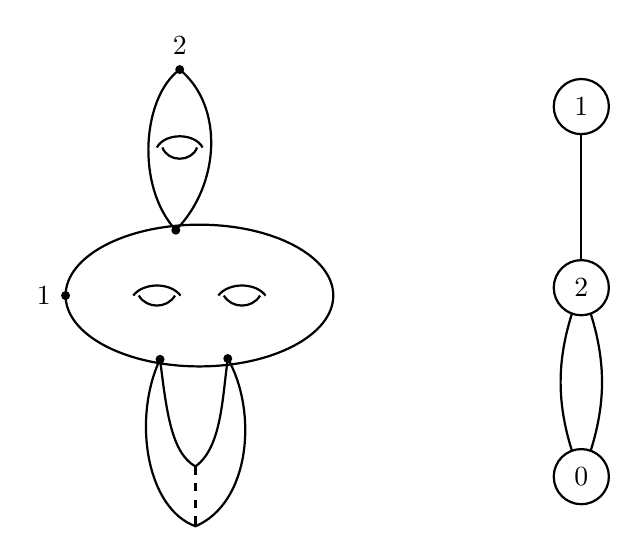
\begin{tikzpicture}[
        x=1cm,
        y=1cm,
        curve component/.style={thick},
        marked point/.style={circle,fill=black,inner sep=1.15pt},
        graph vertex/.style={
            circle,draw,thick,fill=white,minimum size=7mm,inner sep=0pt
        }
    ]
        % A three-component curve with components of genera 1, 2, and 0.
        \draw[curve component] (1.5,3.65) ellipse [x radius=1.7,y radius=0.9];

        % The two handles on the genus-two component.
        \draw[curve component]
            (0.66,3.65)
            .. controls (0.79,3.82) and (1.13,3.82) .. (1.26,3.65);
        \draw[curve component]
            (0.73,3.65)
            .. controls (0.83,3.48) and (1.09,3.48) .. (1.19,3.65);
        \draw[curve component]
            (1.74,3.65)
            .. controls (1.87,3.82) and (2.21,3.82) .. (2.34,3.65);
        \draw[curve component]
            (1.81,3.65)
            .. controls (1.91,3.48) and (2.17,3.48) .. (2.27,3.65);

        % The genus-one component attached above.
        \coordinate (uppernode) at (1.2,4.48);
        \draw[curve component]
            (uppernode)
            .. controls (0.68,5.05) and (0.78,6.18) .. (1.25,6.52)
            .. controls (1.82,6.05) and (1.76,5.05) .. cycle;
        \draw[curve component]
            (0.96,5.53)
            .. controls (1.06,5.72) and (1.44,5.72) .. (1.54,5.53);
        \draw[curve component]
            (1.03,5.53)
            .. controls (1.10,5.34) and (1.40,5.34) .. (1.47,5.53);

        % The rational component attached at two nodes below.
        \coordinate (lowerleft) at (1.00,2.84);
        \coordinate (lowerright) at (1.86,2.85);
        \draw[curve component]
            (lowerleft)
            .. controls (0.65,2.10) and (0.82,0.95) .. (1.45,0.72)
            .. controls (2.15,1.02) and (2.24,2.18) .. (lowerright);
        \draw[curve component]
            (lowerleft)
            .. controls (1.08,2.20) and (1.14,1.65) .. (1.45,1.48)
            .. controls (1.78,1.72) and (1.79,2.34) .. (lowerright);
        \draw[curve component,dashed] (1.45,1.48) -- (1.45,0.72);

        % Nodes and marked points.
        \node[marked point] at (uppernode) {};
        \node[marked point] at (lowerleft) {};
        \node[marked point] at (lowerright) {};
        \node[marked point,label=left:{$1$}] at (-0.2,3.65) {};
        \node[marked point,label=above:{$2$}] at (1.25,6.52) {};

        % The dual graph: the vertex labels record the genera.
        \coordinate (vone) at (6.35,6.05);
        \coordinate (vtwo) at (6.35,3.75);
        \coordinate (vzero) at (6.35,1.35);
        \draw[curve component] (vone) -- (vtwo);
        \draw[curve component]
            (vtwo) to[out=-112,in=112] (vzero);
        \draw[curve component]
            (vtwo) to[out=-68,in=68] (vzero);
        \node[graph vertex] at (vone) {$1$};
        \node[graph vertex] at (vtwo) {$2$};
        \node[graph vertex] at (vzero) {$0$};
    \end{tikzpicture}
    \end{center}
\end{exm}

对对数或穿孔 R-映射
\begin{equation*}
\begin{tikzcd}
    & \mf{P} \ar{d} \\
    C \ar{ur}{f} \ar{d} \ar{r} & B \C_{\omega}^{\times} \\
    S,
\end{tikzcd}
\end{equation*}
我们通过取整个图的相伴广义锥复形将其热带化。因 \(B \C_{\omega}^{\times}\) 无对数结构，所见为
\begin{equation*}
\begin{tikzcd}
    \Sigma(C) \ar{d} \ar{r}{\Sigma(f)} & \Sigma(\mf{P}) = \R_{\geq 0} \\
    \Sigma(S).
\end{tikzcd}
\end{equation*}
现设 \(S = \Spec (Q \to \C)\) 为对数点，其中 \(Q\) 为 fs sharp 幺半群。特别地，这意味着 \(\Sigma(S) = Q_{\R}^{\vee}\)。因一切皆（分片）线性，只需考虑内点 \(t \in \Sigma(S)\) 并考虑 \(\Sigma(C)_t\)。

每条半边视为从所附顶点向外指，特别地，这意味着到 \(\R_{\geq 0}\) 的线性映射对应于斜率。我们称之为\textit{接触阶}。特别地，若 \(h \neq \hat{h}\) 经 \(\imath\) 相关，则有 \(c(h) = - c(\hat{h})\)。对一切 \(v \in \V\)，还定义\textit{退化度}
\[ e_v \colon Q_{\R}^{\vee} \to \R_{\geq 0} \qquad t \mapsto \Sigma(f)_t (v). \]
特别地，\(e_v \in Q\) 为整点。

接下来需引入穿孔腿。记为
\[ \L^{\circ} = \ab\{ h \in \H \mid \Sigma(f)_t(h) \text{ is bounded and nontrivial for all } t \in Q_{\R}^{\vee}\}. \]
在 \(h \in \L^{\circ}\) 处定义预稳定使 \(0 \in \ol{\Sigma(f)_t(h)}\)，这是技术上必要的假设。在一切穿孔腿皆预稳定的假设下，可定义\textit{边长}函数
\[ \ell \colon \E \cup \L^{\circ} \to \ms{Map}(Q_{\R}^{\vee}, \R_{\geq 0}) \qquad x \mapsto \ell(x) \colon t \mapsto \ell(x)(t). \]
注意对边 \(E\)，\(\ell(E) \in Q\) 亦为整点。对穿孔腿，在细分之下亦然。

\subsection{对数 GLSM 不变量}%
\label{sub:Log GLSM invariants}

\begin{defn}
    定义对数映射 \(f\) 的\textit{装饰热带型}为
    \[ \bm{\tau} = (G, c \colon \H \to \Z, \beta \colon \V \to H_2(X)). \]
\end{defn}

\begin{defn}
    对数或穿孔映射 \(f\) 称为\textit{紧型}，若
    \begin{enumerate}
        \item 对一切 \(t\)，\(\Ima \Sigma(f)_t\) 有界；
        \item 对一切接触阶为 \(0\) 的半边 \(h\)，有 \(f(p_h) \in 0_{\mf{P}}\)。
    \end{enumerate}
\end{defn}

现可定义 fs 对数概形范畴 \(\ms{LogSch}\) 上以 \(\tau\) 为标记的稳定穿孔 R-映射范畴 \(\mc{R}(\mf{P}, \tau)\)。

\begin{thm}[{\cite{CJR2021,CJRpunctured}}]
    栈 \(\mc{R}(\mf{P},\bm{\tau})\) 由带基本/极小对数结构的正常 DM 栈表出。
\end{thm}

\begin{rmk}
    若 \(\V = \ab\{v\}\) 为单点集，则记为
    \[ \mc{R}_{g, c}(\mf{P}, \beta) \coloneqq \mc{R}(\mf{P}, \bm{\tau}). \]
\end{rmk}

考虑下图
\begin{equation*}
\begin{tikzcd}
    & \mf{P} \ar{d} \\
    \mc{C} \ar{ur}{f} \ar{d}{\pi} \ar{r} & B \C_{\omega}^{\times} \\
    \mc{R},
\end{tikzcd}
\end{equation*}
其中设 \(\mc{R} \coloneqq \mc{R}(\mf{P}, \bm{\tau})\)。则完美阻碍理论定义为
\[ T_{\mc{R}/\ms{Log}_{\mf{M}_G}} \to \E_{\square} = R \pi_* f^* T_{\mf{P}/B\C_{\omega}^{\times}}. \]
此处两切丛皆指对数切复形。由此完美阻碍理论定义典范虚拟圈
\[ [\mc{R}(\mf{P}, \bm{\tau})]^{\vir}. \]
此虚拟圈的主要缺点是不能复现 Gromov-Witten 理论。然而可考察它与 GW 理论的差异，但为此需要双有理修改。设 \(Q\) 为 sharp 幺半群。它有偏序：若存在非零 \(c \in Q\) 使 \(a+c = b\)，则 \(a < b\)。

\begin{defn}
    称 \(f\) 或 \(\Sigma(f)\) 具有\textit{一致极大退化}，若存在 \(e_{\max} \in \ab\{e_v \mid v \in \V \}\) 使对一切 \(v \in \V\) 有 \(e_{\max} \geq e_v\)。
\end{defn}

\begin{rmk}
    若 \(f\) 为紧型且具一致极大退化，则 \(\Sigma(f)\) 被 \(e_{\max}\) 一致有界。
\end{rmk}

\begin{defn}
    定义 \(\mc{U}(\mf{P}, \bm{\tau})\) 为以 \(\bm{\tau}\) 为标记具一致极大退化的稳定穿孔或对数 R-映射栈。
\end{defn}

\begin{rmk}
    若 \(\V = \ab\{v\}\) 为单点集，则记为
    \[ \mc{U}_{g, c}(\mf{P}, \beta) \coloneqq \mc{U}(\mf{P}, \bm{\tau}). \]
    若其中一个接触阶为负，则记为
    \[ \mc{U}_{g, c}(\infty, \beta) \coloneqq \mc{U}(\mf{P}, \bm{\tau}). \]
\end{rmk}

注意顶点有两类：若顶点映到 \(0\)，则要么至少有一条半边指向上方，要么一切接触阶皆为 \(0\)，此时皆收缩。这些称为\textit{对数顶点}。另一类顶点是不映到 \(0\) 的。要么一切半边皆指向下方，要么有些半边指向上方。这些称为\textit{\(\infty\)-顶点}。而且，紧型的顶点即无指向上方半边的顶点。

若忘掉一致极大退化条件，则有映射
\[ \mc{U}(\mf{P}, \bm{\tau}) \xrightarrow{F} \mc{R}(\mf{P}, \bm{\tau}) \]
它是 \(\ms{LogSch}\) 上的子范畴。然而，作为代数栈的态射，它是对数 \'etale、正常满射。此外，\(\mc{U}\) 有从 \(\mc{R}\) 拉回的典范完美阻碍理论。在顶点集为单点集时，有
\begin{align*}
    F_* [\mc{U}_{g, c}(\mf{P}, \beta)]^{\vir} &= [\mc{R}_{g, c}(\mf{P}, \beta)]^{\vir}; \\
    F_* [\mc{U}_{g, c}(\infty, \beta)]^{\vir} &= [\mc{R}_{g, c}(\infty, \beta)]^{\vir}.
\end{align*}
在对数顶点情形，事实上由带 p-场的稳定映射模空间有包含
\begin{equation*}
\begin{tikzcd}
    \mc{U} \ar{rr}{F} & & \mc{R} \\
    & \mc{R}_{g,c}(\mf{P}^{\circ}, \beta) \ar[hookrightarrow]{ul} \ar[hookrightarrow]{ur}.
\end{tikzcd}
\end{equation*}
若以 \(\mc{R}^{\circ}\) 记 p-场模空间，则边界
\[ \Delta \coloneqq \mc{U} \setminus \mc{R}^{\circ} \]
为 Cartier 除子。由一致极大退化条件，有截面
\[ e_{\max} \in H^0(\bar{M}_{\mc{U}}). \]
这等价于态射
\[ \mc{U} \to ([\A^1/\G_m], 0) \]
将 \(0\) 拉回到 \(\Delta\) 的数据。

我们定义\textit{超势}为函数
\begin{equation*}
\begin{tikzcd}
    \mf{P}^{\circ} \ar{rr}{W} \ar{dr} && \mc{L}_{\omega} \ar{dl} \\
    & B \C_{\omega}^{\times}.
\end{tikzcd}
\end{equation*}
其\textit{临界轨迹}记为
\[ \on{Crit}(W) = (\d{W} = 0). \]
若 \(\on{Crit}(W) \to B\C_{\omega}^{\times}\) 正常，则称 \(W\) 具\textit{正常临界轨迹}。

例如，设关心 GW 理论。设 \(X\) 为光滑射影簇，\(V\) 为 \(X\) 上的向量丛，\(s \in H^0(V)\)。设 \(Z = (s = 0)\)。则得到
\[ W \colon \mf{P}^{\circ} = V^{\vee} \boxtimes \mc{L}_{\omega} \xrightarrow{s \otimes 1_{\omega}} \mc{L}_{\omega}. \]

\begin{lem}
    \(W\) 具正常临界轨迹当且仅当 \(Z\) 光滑且余维为期望值。
\end{lem}

\begin{exm}
    设 \(X\) 为一点，\(V = \C\)，\(s \neq 0\)。则 \(\d{W} = s \neq 0\)，故临界轨迹为空。
\end{exm}

用 Kiem--Li 余截面局部化方法~\cite{KiemLi2013}，可得虚拟圈
\[ [\mc{R}_{g, c=n}(\mf{P}^{\circ}, \beta)]_W^{\vir}, \]
它支于临界轨迹上。在 GW 理论中，它等于 GW 虚拟圈，
\[ \pm [\bar{M}_{g,n}(\on{Crit}(W), \beta)]^{\vir}, \]
其中符号可显式计算。

\begin{thm}[{\cite{CJR2021,CJW2021}}]
    设 \(\bm{\tau}\) 为紧型。在紧型设定下，
    \begin{enumerate}
        \item \(\mc{U}(\mf{P}, \bm{\tau})\) 具有约化完美阻碍理论，给出约化虚拟圈 \([\mc{U}(\mf{P}, \bm{\tau})]^{\vir}\)；
        \item \(\Delta\) 具有约化完美阻碍理论，给出约化虚拟圈 \([\Delta]^{\vir}\)；
        \item 在单对数顶点情形有 \([\mc{U}_{g, c=n}(\mf{P}, \beta)]^{\on{red}} = \pm [\bar{M}_{g,n}(\on{Crit}(W), \beta)]^{\vir}\)。而且，有公式
            \[ [\mc{U}_{g, c=n}(\mf{P}, \beta)]^{\on{red}} = [\mc{U}_{g, c=n}(\mf{P}, \beta)]^{\vir} - \tilde{r} [\Delta]^{\on{red}}, \]
            其中 \(\tilde{r}\) 为 \(W\) 沿 \(\infty\) 的极点阶。
    \end{enumerate}
\end{thm}

\subsection{热带分解与有限生成}%
\label{sub:Tropical decomposition and finite generation}

以下热带分解及其应用来自工作草稿~\cite{CJRtropical2025}。有效不变量及其公理在~\cite{CJRpunctured} 中建立。

从现在起，考虑较简单设定，其中 \(X\) 为光滑射影簇，\(V\) 为 \(X\) 上的线丛。此时设 \(Z = (s = 0)\) 光滑余维 \(1\)。而且设 \(Z\) 为 Calabi-Yau 三维流形。考虑不变量
\[ N_{g, \beta} \coloneqq \int_{[\bar{M}_{g,0}(Z, \beta)]^{\vir}} 1 \in \Q \]
与生成级数
\[ F_g = \sum_{\beta \geq 0} N_{g, \beta} Q^{\beta} \in \Lambda \coloneqq \C \ps{Q}. \]

\begin{conj}[Yamaguchi-Yau, Alim-L\"ange {\cite{YY2004,AlimLange2007}}]
    设 \(g=0\) 镜像对称对 \(Z\) 成立。则存在有限生成 \(\Q\)-代数 \(R \subset \Lambda\) 使对一切 \(g \geq 2\) 有 \(F_g \in (I_0(q))^{2g-2} R\)。
\end{conj}

我们的主要目标是如下。

\begin{thm}[{\cite{CJRtropical2025}}]
    设 \(Z\) 为 Fano 四维流形 \(X\) 中无奇上同调的 Calabi-Yau 三维流形超曲面。设 \(\{\phi_j\}\) 为 \(H^*(X)\) 的基，\(\ab\{\phi^j\}\) 为对偶基。则对一切 \(g \geq 0\) 有
    \begin{align*}
        &F_g = (-1)^{1-g} \sum_{\tau' \in G_g'} \frac{(-1)^{\abs{\V_{\infty}}}}{\abs{\Aut(\tau')}} \cdot \prod_{E \in \E} c(E) \\
        & \cdot \sum_{j_E \mid E = \ab\{E_{\log}, E_{\infty}\} \in \E} \prod_{\substack{v \in \V_{\infty} \\ g(v)=1 \\ \H_v = \ab\{E_{\infty}\}}} c_1^{\mr{eff}}(\phi^{j_E}) \cdot \prod_{\substack{v \in \V_{\infty} \\ g(v) \geq 2}} \tilde{Q}^{\beta(v)} \cdot \exp \ab(\int_{\beta(v)} K(Q) )  \\
        & \cdot \ab(\prod_{E_{\infty} \in \H_v'}\int_{\beta(v)} \phi^{j_E}) \cdot c_{g(v), \beta(v)}^{\on{eff}} 
         \cdot \prod_{v \in \V_{\log}} \Omega_{g(v), \abs{\H_1(v)}, \abs{\H_2(v)}} (\phi_{j_E} \colon E_{\log} \in \H_1(v)).
    \end{align*}
\end{thm}

\begin{exm}
    设 \(Y\) 为带环面对数结构的环面簇。则 \(\Sigma(Y)\) 为视为锥复形的环面扇，可考虑其边界 \(\Delta_Y = \sum_{\rho \in \Sigma(Y)^1} \Delta_{\rho}\)。
\end{exm}

若考虑 \([\Delta]^{\on{red}}\)，应得类似公式
\[ [\Delta]^{\on{red}} = \sum_{\rho \in \Sigma(\Delta)(1)} [\Delta_{\rho}]^{\on{red}}. \]
问题是 \(\rho\) 代表什么。事实上，它们参数化刚性热带曲线。在热带化
\begin{equation*}
\begin{tikzcd}
    \Sigma(C)_{\rho} \ar{d} \ar{r} & \Sigma(\mc{C}) \ar{r}{f} \ar{d} & \R_{\geq 0} \\
    \rho \ar[hookrightarrow]{r} & \Sigma(\mc{U}),
\end{tikzcd}
\end{equation*}
中，可见 \(f_{\rho}\) 刚性当且仅当源热带曲线为二部图，其中一组顶点映到 \(e_{\max}\) 而另一组顶点映到 \(0\)。

\begin{exm}
    设 \(X\) 为一点且 \(Z = \emptyset\)。又考虑 \(g = 2, n = 0\)。则可能的图见~\Cref{fig:tropgraphs}。
    \begin{figure}[htpb]
    \begin{center}
    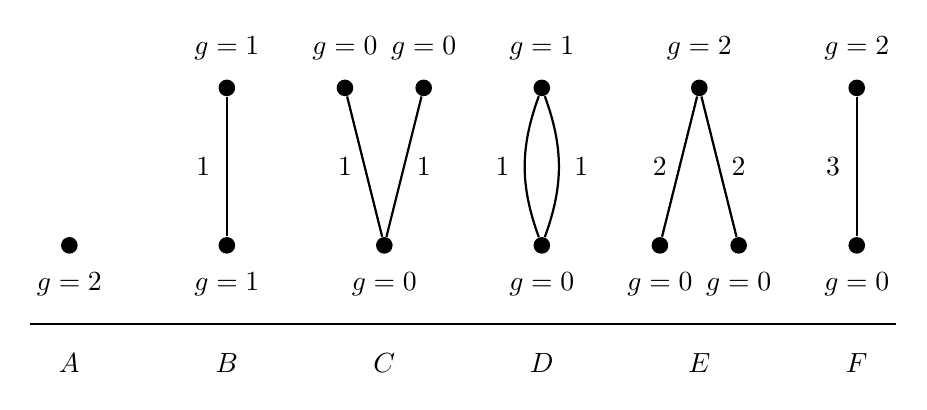
\begin{tikzpicture}[scale=1, transform shape]
        \node[fill=black,circle,minimum size=6pt,inner sep=0pt] (A) at (0,0) {};
        \node[fill=black,circle,minimum size=6pt,inner sep=0pt] (B1) at (2,0) {};
        \node[fill=black,circle,minimum size=6pt,inner sep=0pt] (B2) at (2,2) {};
        \node[fill=black,circle,minimum size=6pt,inner sep=0pt] (C1) at (4,0) {};
        \node[fill=black,circle,minimum size=6pt,inner sep=0pt] (C2) at (3.5,2) {};
        \node[fill=black,circle,minimum size=6pt,inner sep=0pt] (C3) at (4.5,2) {};
        \node[fill=black,circle,minimum size=6pt,inner sep=0pt] (D1) at (6,0) {};
        \node[fill=black,circle,minimum size=6pt,inner sep=0pt] (D2) at (6,2) {};
        \node[fill=black,circle,minimum size=6pt,inner sep=0pt] (E1) at (8,2) {};
        \node[fill=black,circle,minimum size=6pt,inner sep=0pt] (E2) at (7.5,0) {};
        \node[fill=black,circle,minimum size=6pt,inner sep=0pt] (E3) at (8.5,0) {};
        \node[fill=black,circle,minimum size=6pt,inner sep=0pt] (F1) at (10,0) {};
        \node[fill=black,circle,minimum size=6pt,inner sep=0pt] (F2) at (10,2) {};
        \draw[-,thick] (B1) -- (B2);
        \draw[-,thick] (C2) -- (C1) -- (C3);
        \draw[-,thick] (D1) edge[bend left=20] (D2);
        \draw[-,thick] (D2) edge[bend left=20] (D1);
        \draw[-,thick] (E2) -- (E1) -- (E3);
        \draw[-,thick] (F1) -- (F2);
        \node at (0,-0.5) {$g=2$};
        \node at (2,-0.5) {$g=1$};
        \node at (4,-0.5) {$g=0$};
        \node at (6,-0.5) {$g=0$};
        \node at (7.5,-0.5) {$g=0$};
        \node at (8.5,-0.5) {$g=0$};
        \node at (10,-0.5) {$g=0$};
        \node at (2,2.5) {$g=1$};
        \node at (3.5,2.5) {$g=0$};
        \node at (4.5,2.5) {$g=0$};
        \node at (6,2.5) {$g=1$};
        \node at (8,2.5) {$g=2$};
        \node at (10,2.5) {$g=2$};
        \draw[-,thick] (-0.5,-1) -- (10.5,-1);
        \node at (0,-1.5) {$A$};
        \node at (2,-1.5) {$B$};
        \node at (4,-1.5) {$C$};
        \node at (6,-1.5) {$D$};
        \node at (8,-1.5) {$E$};
        \node at (10,-1.5) {$F$};
        \node at (1.7,1) {$1$};
        \node at (3.5,1) {$1$};
        \node at (4.5,1) {$1$};
        \node at (5.5,1) {$1$};
        \node at (6.5,1) {$1$};
        \node at (7.5,1) {$2$};
        \node at (8.5,1) {$2$};
        \node at (9.7,1) {$3$};
    \end{tikzpicture}
    \end{center}
        \caption{Graphs of tropical types for $X = \mr{pt}$ and \(Z = \emptyset\) when $g=2$.}%
    \label{fig:tropgraphs}
    \end{figure}
\end{exm}

\begin{thm}[Tropical quantum Lefschetz {\cite{CJRtropical2025}}]
    设 \(X\) 与 \(Z\) 如前。对任何 \(\beta \in H_2(X)\)、任何 \(\alpha_1, \ldots, \alpha_n \in H^*(X)\) 与任何 \(k_1, \ldots, k_n \in \N\)，有
    \begin{align*}
        \int_{[\bar{M}_{g,n}(Z,\beta)]^{\vir}} \prod_{j=1}^n \ev_j^* (\alpha_j) \psi^{k_j}={}& (-1)^{1-g+\beta \cdot Z} \cdot \sum_{\tau \vdash (g,n,\beta)} \frac{(-1)^{\abs{\V_{\infty}}}}{\abs{\Aut(\tau)}} \cdot \prod_{E \in \E} c(E) \\
        & \cdot \sum_{\ab\{j_E \mid E = \ab\{E_{\log}, E_{\infty}\}\}}  \prod_{v \in \V_{\infty}} \int_{[\mc{U}_v]^{\on{red}}} \prod_{E_{\infty} \in \H_v} \ev_{E_{\infty}}^* \phi^{j_E}  \\
        &  \cdot \prod_{v \in \V_{\log}} \int_{[\mc{R}_v]^{\vir}} \prod_{E_{\log}} \ev_{E_{\log}}^* (\phi_{j_E}) \cdot \prod_{h \in \L_v} \ev_h^* \alpha_h \cdot \psi_h^{k_h} .
    \end{align*}
\end{thm}

\begin{rmk}
    还有虚拟局部化公式，见~\cite{CJRlocalization} 中宣布，可应用于约化理论（仅带 R-环面作用）或典范理论（可应用于环境空间的全体自同构）。
\end{rmk}

现考虑 \(\infty\)-顶点。设 \(\tau_v = (g, c, \beta)\) 并设 \(\mc{U}_v = \mc{U}_{g,c}(\infty, \beta)\)。则第一个计算是
\begin{align*}
    \on{red}\dim \mc{U}_v &= \chi(f^* T_{\mf{P}/B \C^{\times}_{\omega}}) + 1 + \on{trop}\dim  \\
    &= \vir\dim \bar{M}_{g,n}(Z, \beta) + \sum_{h \in \H } (c(h) + 1),
\end{align*}
其中热带维数为 \(3g-4+n\)。注意一切接触阶皆为负，故第二项至多为零。特别地，已证明
\begin{cor}[{\cite{CJRpunctured}}]
    若 \(\vir\dim \bar{M}_{g,n}(Z,\beta) < 0\)，则 \([\mc{U}_v]^{\on{red}} = 0\)。
\end{cor}
还有\textit{平衡条件}，即
\begin{equation}\label{eqn:balancing condition}
    \sum_{h \in \H} c(h) = \deg f^* \mc{O}(\infty) = \int_{\beta} c_1(V) - (2g-2+n).
\end{equation}
这可改写为
\[ 0 \geq \sum_{h \in \H} (c(h)+1) = \int_{\beta} c_1(V) - (2g-2). \]
\begin{prop}[{\cite{CJRpunctured}}]
    可见在如下情形不存在 \(\infty\)-顶点：
    \begin{enumerate}
        \item 有 \(g = 0\) 且 \(V\) nef；
        \item 有 \(g=1\) 且 \(V\) ample，除非 \(\beta = 0\) 且一切 \(c(h) = -1\)。
    \end{enumerate}
\end{prop}

\begin{defn}
    若标记点的接触阶为 \(-1\)，则称该标记为\textit{单位}。
\end{defn}

\begin{notn}
    以 \(\1\) 记单位分支，并记 \(\tau_{v+\1} = (g, c+\1, \beta)\)、\(\mc{U}_{v+\1} = \mc{U}_{g, c+\1}(\infty, \beta)\) 与 \(\mc{R}_{v+\1} = \mc{R}_{g, c+\1}(\infty, \beta)\)。
\end{notn}

\begin{thm}[{\cite[Theorems~1.16--1.17]{CJRpunctured}}]\leavevmode
    \begin{enumerate}
        \item 有映射 \(F_{\1} \colon \mc{U}_{v+\1} \xrightarrow{s} \mc{C}^{\circ} \xrightarrow{\pi} \mc{U}_v\)，其中 \(s\) 双有理；
        \item 有约化虚拟圈等式 \(s_* [\mc{U}_{v+\1}]^{\on{red}} = \pi^* [\mc{U}_v]^{\on{red}}\)；
        \item 若 \(D\) 为 \(X\) 上的除子，则 \(F_{\1 *} (\ev_{\1}^* D \cap [\mc{U}_{v+\1}]^{\on{red}}) = \ab(\int_{\beta} D) [\mc{U}_v]^{\on{red}}\)；
        \item 考虑下图
            \begin{equation*}
            \begin{tikzcd}
                \mc{U}_{v+\1} \ar{r}{F} \ar{d}[swap]{F_{\1}} & \bar{M}_{g,n+1} \ar{d}[swap]{p} \\
                \mc{U}_v \ar{r}{F} & \bar{M}_{g,n}.
            \end{tikzcd}
            \end{equation*}
            则 \(F_* [\mc{U}_{v+\1}]^{\on{red}} = p^* F_* [\mc{U}_v]^{\on{red}}\)。
    \end{enumerate}
\end{thm}

\begin{exm}
    考虑 \(g = 1\) 且 \(Z_d \subset X = \P^N\) 为超曲面的设定。只需考虑 \(\beta = 0\) 且对一切 \(h \in \H\) 有 \(c(h) = -1\)。则可见
    \[ \prod_h \ev_h^* \alpha_h \cdot [\mc{U}_{1,c}(\infty,\beta)]^{\mr{red}} = \ev_{h^{\star}}^* \ab(\prod_h \alpha_h) \cap [\mc{U}_{1,\1}(\infty,\beta)]^{\on{red}}. \]
\end{exm}

\begin{prop}[{\cite{CJRpunctured}}]
    事实上，有
    \[ \mc{U}_{1,\1}(\infty, 0) \simeq \mc{R}_{1,\1}(\infty, 0) \]
    与等式
    \[ [\mc{U}_{1,\1}(\infty, 0)]^{\on{red}} = c_{\dim X} \ab(\mc{H}^{\vee} \boxtimes T_{\mf{P}/B\C_{\omega}^{\times}} + \mc{O} - V). \]
\end{prop}

\begin{exm}
    现考虑五次三维流形 \(Z_5 \subset \P^4\)。则可见 \(\on{red}\dim \mc{U}_v = \sum_{h \in \H} (c(h)+2)\)。单位公理将我们化到 \(c(h) \leq -2\) 的情形。现若一切 \(c(h) = -2\)，须确定需考虑多少新不变量，这等价于求可能的 \(\beta\) 的个数。平衡条件表述为
    \begin{align*}
        \sum_{h \in \H} c(h) &= \int_{\beta} c_1(V) - (2g-2+n) \\
        &= 5\beta - (2g-2+n),
    \end{align*}
    它蕴含 \(0 \geq \sum (c(h)+1) = 5\beta - (2g-2)\)，从而 \(\beta \leq \frac{2g-2}{5}\)。\footnote{This is exactly the number of unknowns predicted if we assume finite generation, the holomorphic anomaly equations, orbifold regularity, and the conifold gap condition.}
\end{exm}

\begin{conj}[Janda {\cite[Conjecture~1.6]{CJRtropical2025}}]\leavevmode
    \begin{enumerate}
        \item 有 \(K(Q) = \log I_0(q) \cdot c_1(K_X^{\vee}) - \frac{I_1}{I_0}\) \\
        \item 典范理论满足 \(\Omega \in I_0(q)^{2g-2+2n_1 + 3 n_2} \cdot R\)。
    \end{enumerate}
\end{conj}

\begin{cor}[{\cite[Theorem~1.7]{CJRtropical2025}}]
    \((X, V)\) 的上述猜想蕴含 \(Z\) 的 Yamaguchi-Yau 有限生成。
\end{cor}
